\chapter{Результаты и их обсуждение}
\label{ch:results}

\section{Экспериментальная установка}
 Для исследования взаимной диффузии газов и измерения коэффициента взаимной диффузии D использовались два сосуда объёмами $V_1$ и $V_2$ ($V_1 \approx V_2 \equiv V $), соединенные трубкой длины $L$ и сечения $S$ (см. рис. 1). Сосуды заполнены смесью двух газов при одинаковом давлении, но с различной концентрацией компонентов. Вследствие взаимной диффузии, проходящей в соединительной трубке, концентрации компонентов в сосудах с течением времени выравнивались. 

Для исключения конвекции обеспечивалось равенство давлений и температур в сосудах до начала измерений. Чтобы считать концентрации газов $n_1$ и $n_2$ внутри каждого сосуда постоянными по всему объёму и принять, что процесс выравниваний концентраций происходил благодаря диффузии в трубке, использовалась соединительная трубка с малым объёмом по сравнению с объёмом сосудов. 

\begin{figure}[ht]
    \centering
        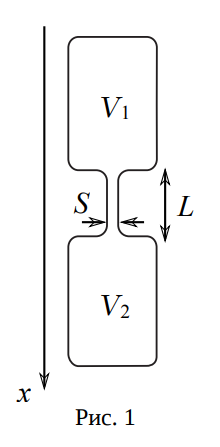
\includegraphics[width = 0.25\textwidth]{img/ustanovka.png}
        
\end{figure}
    \begin{center}
        Рис. 1. Схема установки. Для исследования взаимной диффузии газов и измерения коэффициента взаимной диффузии D использовались два сосуда объёмами $V_1$ и $V_2$ ($V_1 \approx V_2 \equiv V $), заполненные гелием и воздухом при одинаковом давлении, но с различной концентрацией компонентов. Сосуды соединены трубкой длины $L$ и сечения $S$. Чтобы считать концентрации газов $n_1$ и $n_2$ внутри каждого сосуда постоянными по всему объёму и принять, что процесс выравниваний концентраций происходил благодаря диффузии в трубке, использовалась соединительная трубка с малым объёмом по сравнению с объёмом сосудов. Геометрические размеры установки и коэффициент взаимной диффузии гелия и воздуха определяют характерное время выравнивания концентраций между сосудами.  %(полностью описание) для чего, что на рисунке
    \end{center}

    Для нашей установки $\tau$ - характерное время выравнивания концентраций между сосудами, определяется следующей формулой
    
    \begin{equation}
        \label{Tau}
        \tau = \frac{1}{D} \frac{V L}{2S}.
    \end{equation}

    А напряжение на вольтметре удовлетворяет выражению:
    \begin{equation}
        \label{U}
        U = U_0 \, e^{-t / \tau},
    \end{equation}
    где $U_0$ - показание в начальный момент времени (вывод формул смотри в приложении А).

 \section{Обработка результатов измерений}

    Измерили экспериментально зависимость $U(t)$ для рабочих давлений: 40, 60, 80, 100, 120, 160 торр (результаты измерений смотри в Приложении Г.). Для каждого из рабочих давлений построили график зависимости  $ln(U/U_0)(t)$ (см. Рис. 2). 
    
    \begin{figure}[ht]
        \centering
        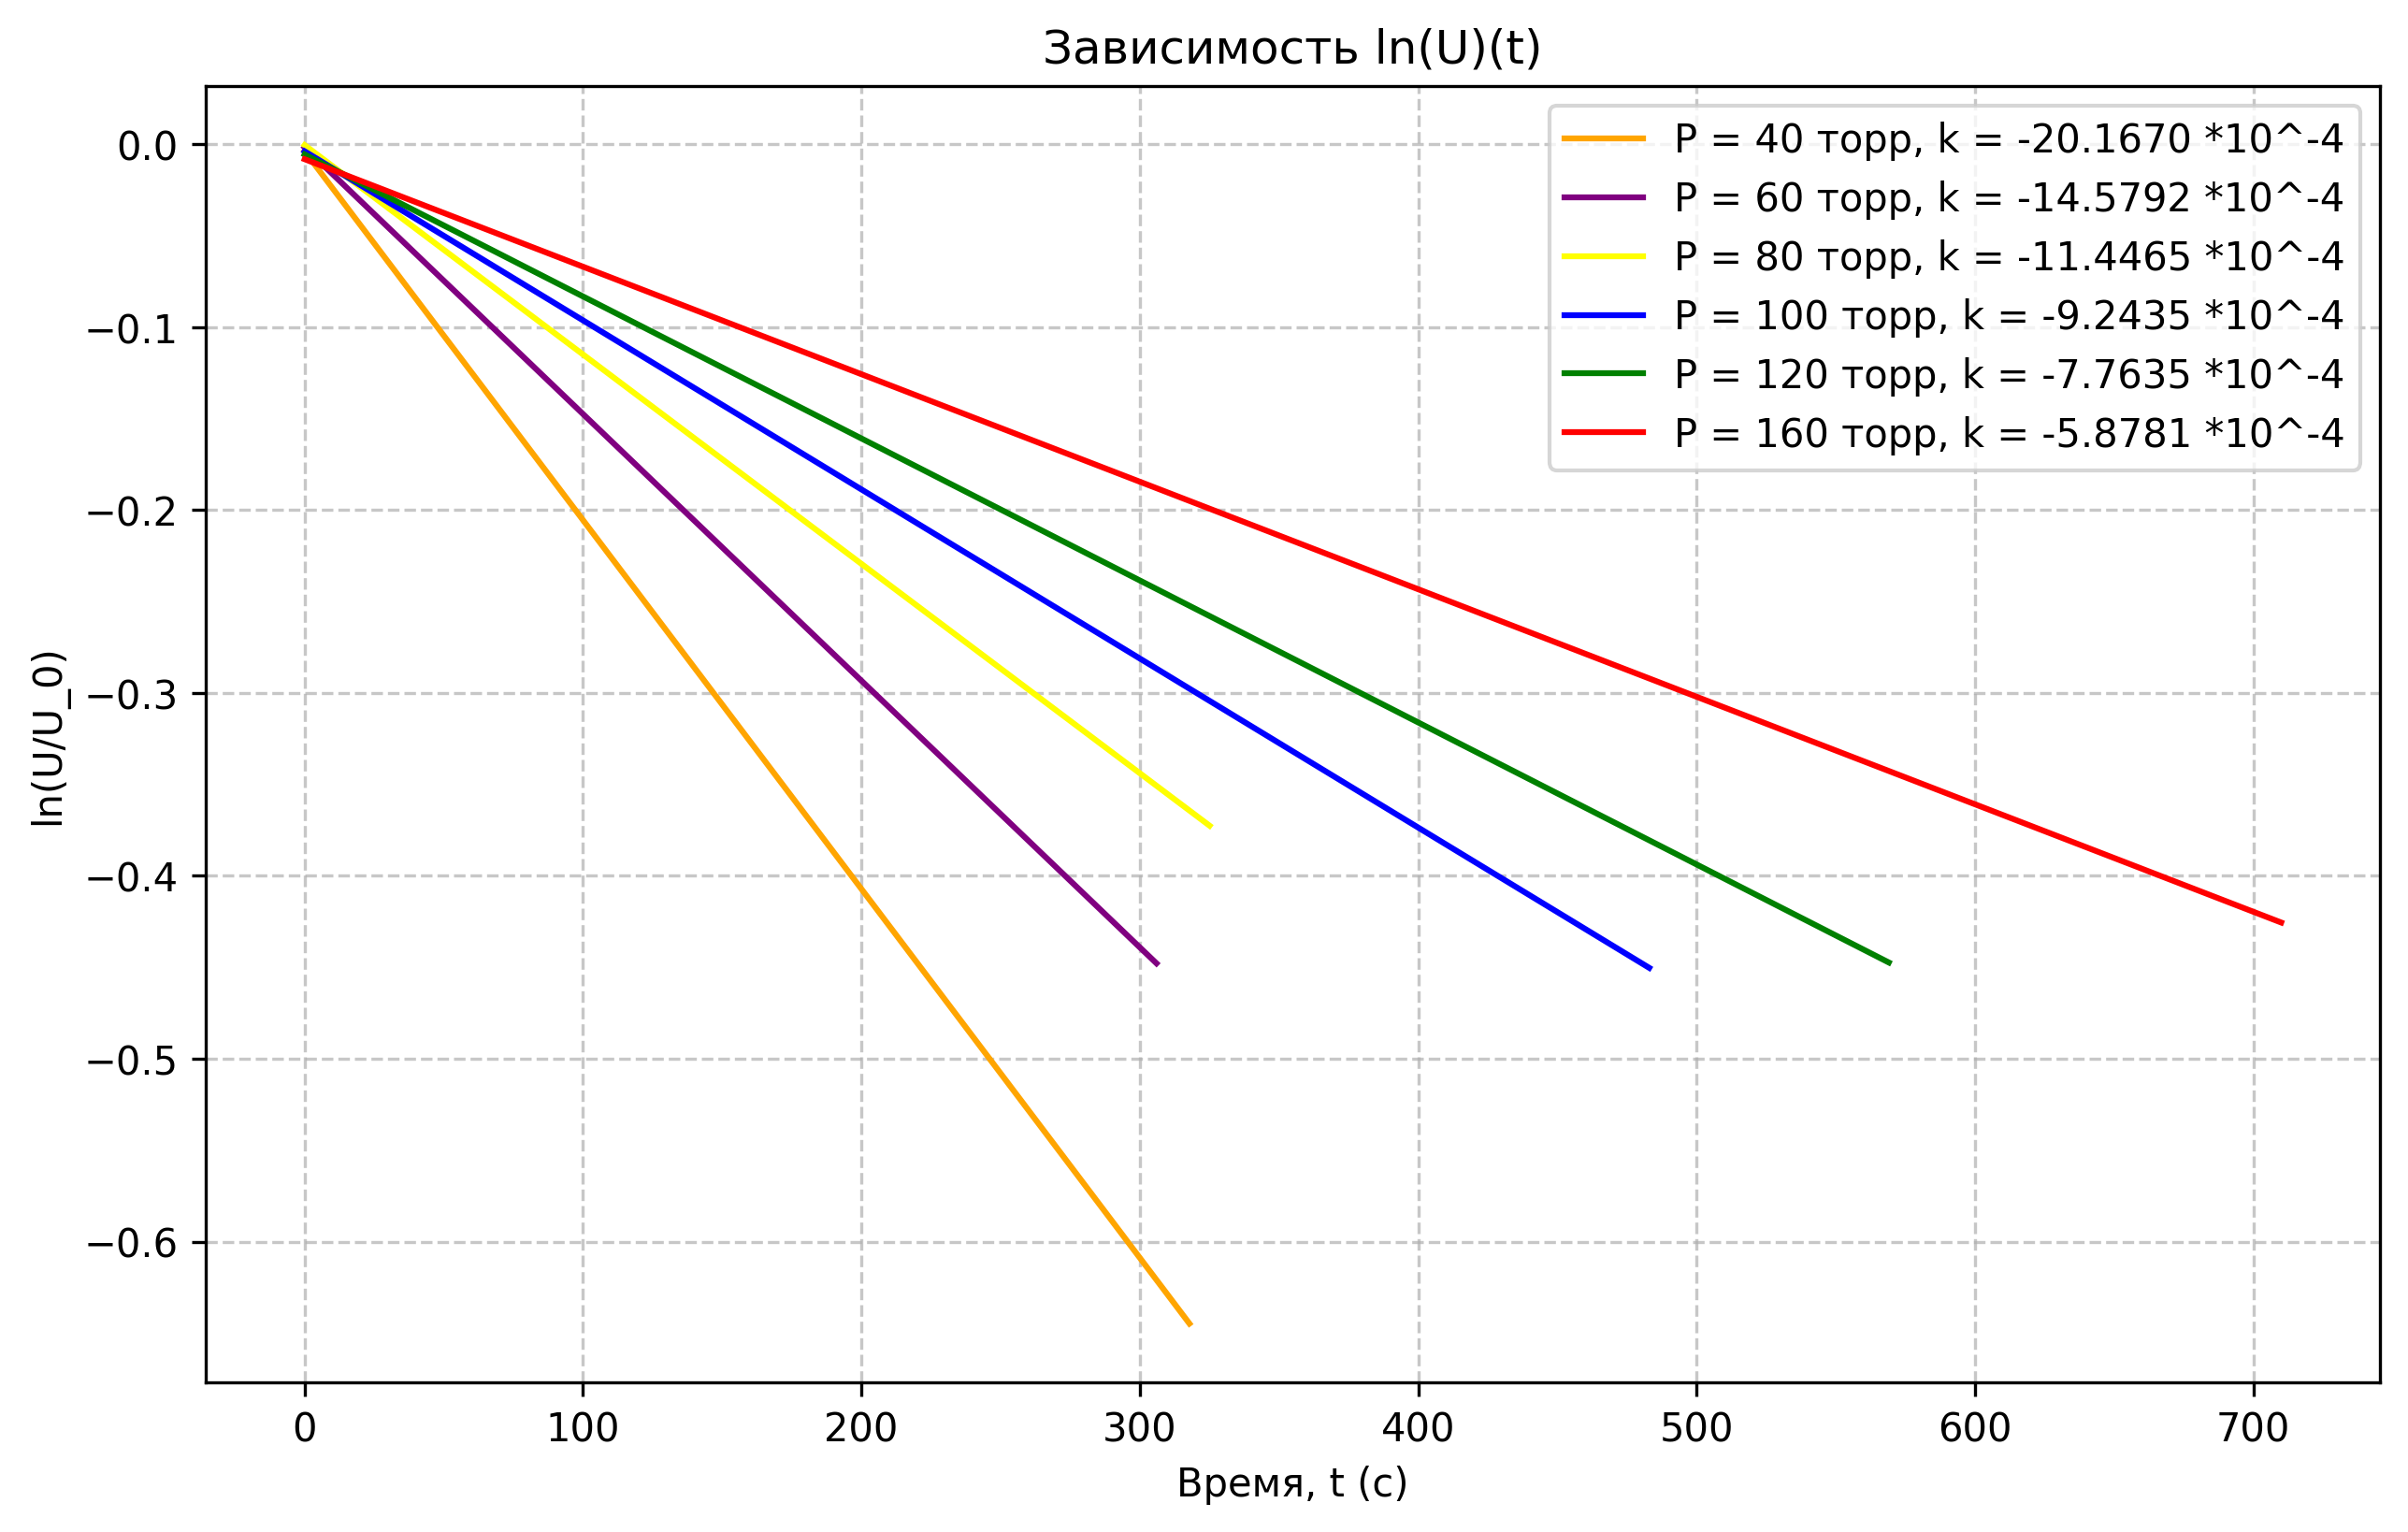
\includegraphics[width = \textwidth]{img/ln(U)(t).png}
    \begin{center}
        Рис. 2. График зависимости $ln(U/U_0) (t)$ для рабочих давлений: 40 (оранжевая линия), 60 (фиолетовая линия), 80 (жёлтая линия), 100 (синяя линия), 120 (зелёная линия), 160 (красная линия). По коэффициенту наклона графика k можно определить величину $1 / \tau$, где $\tau$ - характерное время выравнивания концентраций между сосудами, которая используется для нахождения коэффициента диффузии по формуле (\ref{Tau}).  %(полностью описание) для чего, что на рисунке
    \end{center}
    \end{figure} 
        
    %Измеряя экспериментально зависимость $U(t)$, можно получить характерное время процесса $\tau$, откуда по формуле~(\ref{Tau}) определить коэффициент диффузии $D$.
    
    По угловым коэффициентам и известным геометрическим параметрам установки (см. Приложение В.) рассчитали коэффициенты взаимной диффузии при выбранных рабочих давлениях (формулы (\ref{Tau}) и (\ref{U})). Полученные данные в таблице 1.

\newpage

    \begin{table}[!ht]
        \centering
        \begin{tabular}{|c|c|}
        \hline
            $P, \text{торр}$ & $D, \text{см}^2/c$\\ \hline
            $40  \pm 2$ & $4.14  \pm 0.28$ \\ \hline
            $60  \pm 2$ & $2.99  \pm 0.14$ \\ \hline
            $80  \pm 2$ & $2.35  \pm 0.10$ \\ \hline
            $100 \pm 2$ & $1.90  \pm 0.08$ \\ \hline
            $120 \pm 2$ & $1.59  \pm 0.05$ \\ \hline
            $160 \pm 2$ & $1.21  \pm 0.04$ \\ \hline
        \end{tabular}
        
\vspace{5pt}

        Таблица 1. Результаты расчётов коэффициента диффузии $D$ для каждого значения рабочего давления P
        \label{coeffs}
    \end{table}

    Построили график зависимости коэффициента диффузии от обратного давления в координатах $D(1/P)$. Экстраполируя график к атмосферному давлению, оценили соответствующий коэффициент диффузии.

    \begin{figure}[ht]
        \centering
        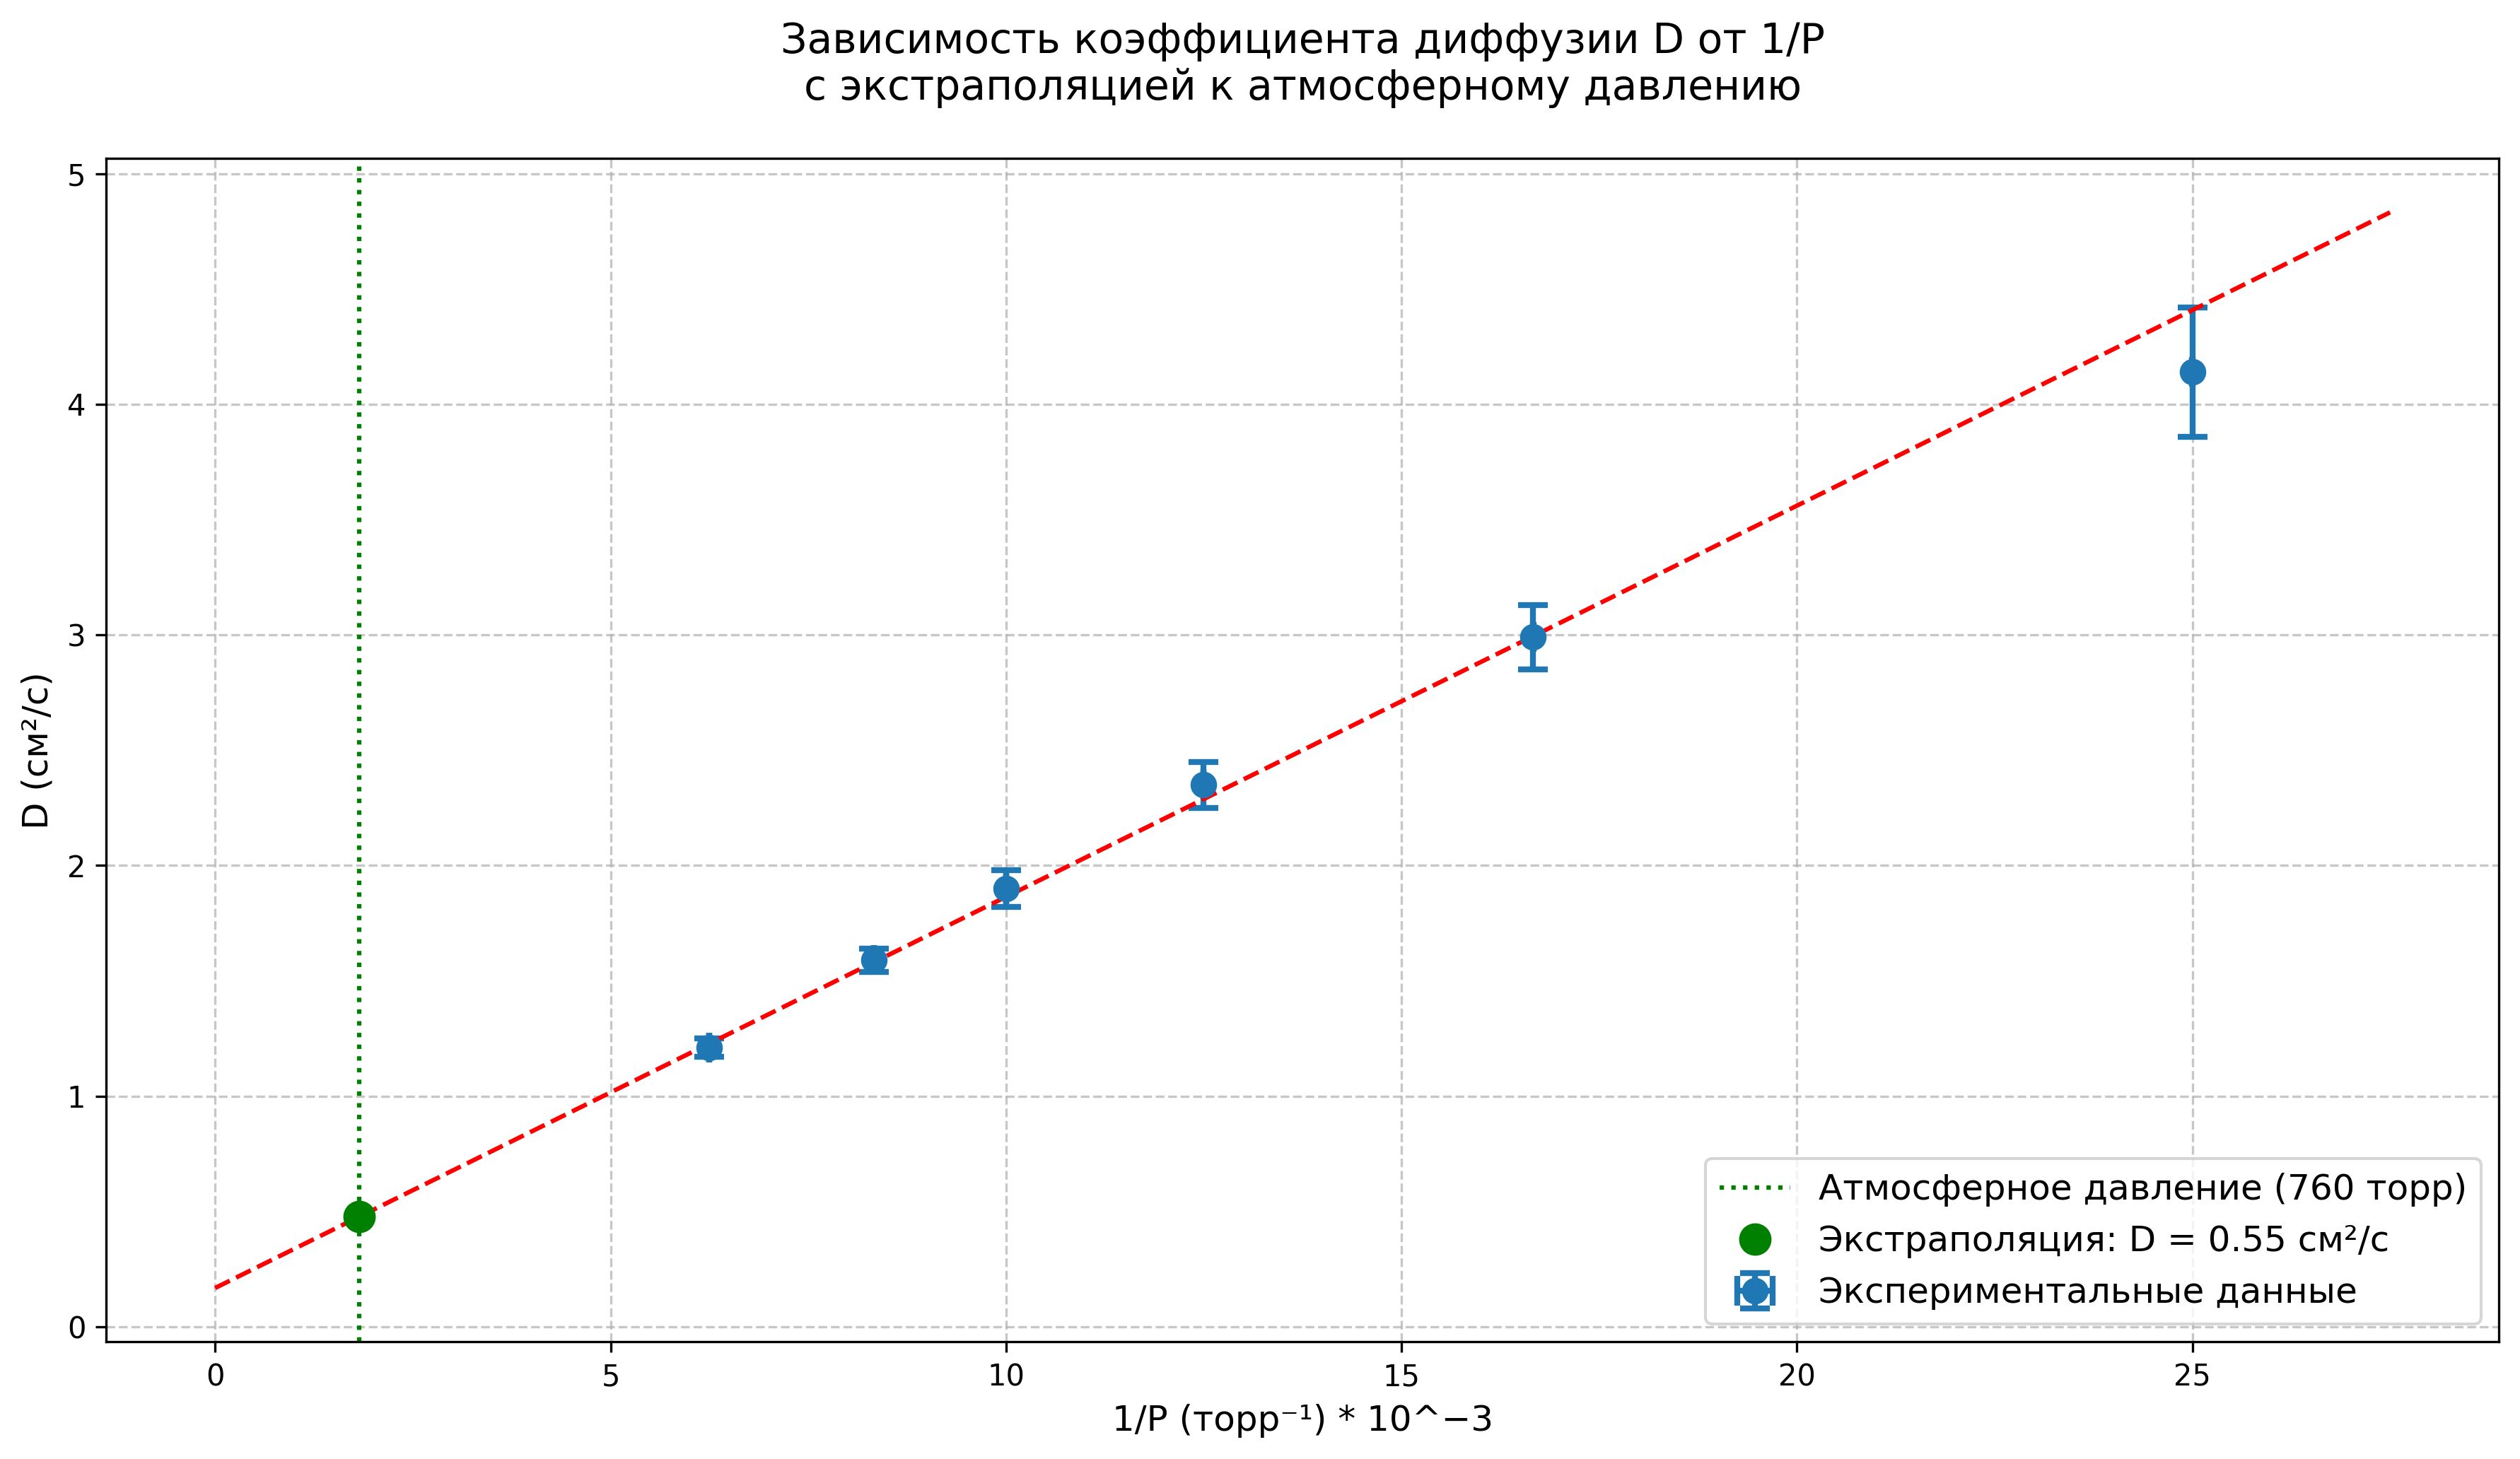
\includegraphics[width = \textwidth]{img/D_vs_invP_extrapolated.png}
    \begin{center}
        Рис. 3. График зависимости коэффициента диффузии D от обратного давления P. Синие точки (кресты) - значения, полученные из экспериментальных данных. Красная пунктирная линия проведена, чтобы показать экстраполяцию к атмосферному давлению. Зелёная пунктирная линия отмечает точки, имеющие атмосферное давление, а большая зелёная точка - это значение полученное при экстраполяции. %(полностью описание) для чего, что на рисунке
    \end{center}
    \end{figure} 

    Коэффициент взаимной диффузии воздуха и гелия при атмосферном давлении получился равным:
    \begin{align*}
        D_{\text{атм}} &= 0.55 \pm 0.08~\text{см}^2/\text{с}\\
    \end{align*}

    Результат совпал с табличным значением $D_{\text{табл}} = 0.62~\text{см}^2/\text{с}$ с учётом погрешности. 